\subsection{Ganho e perda de energia}
Até agora, foram ignorados os efeitos os quais mudam a energia de um elétron armazenado; agora é necessário considerar estes processos onde um elétron ganha ou perde energia. A aceleração lateral ao longo das partes curvas da trajetória faz com que um elétron irradie uma parte da sua energia. As características desta perda por radiação serão discutidas mais a fundo na \autoref{sec:4.1}. Se um elétron deve permanecer capturado no anel de armazenamento, esta perda por radiação deve ser compensada por, na média, um ganho de energia equivalente proporcionado pelo sistema de aceleração de radiofrequência do anel -- um ou mais eletrodos os quais produzem, ao longo de algumas partes da órbita, um campo elétrico que carrega o elétron em movimento. É a ação combinada da perda por radiação com o ganho de energia -- juntamente com as propriedades do campo guia -- que garante a estabilidade dos \textit{bunches} armazenados, além de também ser responsável pelas pequenas oscilações de energia dos elétrons de um \textit{bunch}.

Um elétron com energia nominal $E_0$, movendo-se na órbita ideal, irá irradiar uma certa quantidade de energia, diga-se $U_0$, a cada revolução. Essa perda por radiação será sempre uma epquena fração da energia do elétron (tipicamente da ordem de $10^{-4}$ ou menos). E o ganho de energia do sistema de aceleração é, claro, da mesma ordem de magnitude. A pequena magnitude da perda por radiação em uma revolução permite algumas simplificações na sua análise. Para começar, pode-se aproximar que o elétron que começa uma revolução com energia $E_0$ irá perder a energia $U_0$ em uma revolução. Apesar de que a energia não permanecerá exatamente em $E_0$, nem a trajetória permanecerá na órbita ideal, os desvios em uma revolução podem ser desprezados. Com tudo, os efeitos cumulativos após várias revoluções devem ser levados em consideração.

Se o movimento de um elétron com energia $E_0$ segue uma oscilação betatron, sua taxa instantânea de perda de energia pode mudar -- devido à variação da aceleração lateral ao longo da trajetória. Mas a perda de energia média em uma revolução não irá sofrer alteração para uma aproximação de primeira ordem da amplitude da oscilação. Em outras palavras, mudanças na aceleração lateral são proporcionais a $x$ e irão, considerando apenas termos de primeira ordem, ter média zero em um ciclo completo. Já que basta considerar apenas os efeitos cumulativos de várias oscilações betatron, é necessário apenas analisar a média da perda de energia. Continuando com a análise linear do anel de armazenamento, qualquer dependência entre a perda por radiação e os desvios betatron pode ser ignorada.

No entanto, a perda por radiação irá variar com a variação da energia do elétron. Tanto uma variação na trajetória quanto na energia pode contribuir para uma alteração na perda de energia. Como toda variação de energia é lenta, pode-se considerar que um elétron está se movendo a todo instante na órbita fechada correspondente à sua energia instantânea -- ou está sofrendo oscilações betatron ao redor desta órbita. Como esta órbita fechada já é conhecida, pode-se computar a perda de energia em uma revolução. Por agora, pode-se considerar a perda de energia $U_{rad}(\epsilon)$ é uma função do desvio de energia $\epsilon$.

Como apenas pequenos desvios de energia estão sob análise, pode-se manter apenas termos de primeira ordem ao expandir a função em série de Taylor. Avaliando a expansão em $\epsilon=0$ -- ou seja, em $E=E_0$ -- tem-se que
\begin{align}
	U_{rad} = U_0 + D\epsilon\label{eq:3.23}
\end{align}
onde
\begin{align}
	D = \left(\frac{d\ U_{rad}}{d\ \epsilon}\right)_0
\end{align}
Neste momento, a perda por radiação é descrita pelas constantes $U_0$ e $D$ -- as quais serão avaliadas em termos das propriedades do campo guia na \autoref{sec:4}.

Agora, foque a análise para o sistema de aceleração de radiofrequência -- o sistema de RF, para facilitar -- o qual fornece energia aos elétrons para compensar a perda por radiação. O sistema de RF consiste de uma ou mais cavidades ressonantes, como a que está representada na \autoref{fig:fig30}, situadas em várias partes do anel e alimentadas com uma tensão de RF advinda de fontes de RF sincronizadas. estas cavidades produzem campos elétricos oscilantes ao longo da trajetória dos elétrons; e é a componente destes campos ao longo do caminho do elétron que carrega sua energia. Um elétron que completa um ciclo na órbita ideal é carregado pela cavidade de Rf com uma energia $U_0$ igual a integral da força elétrica instantânea ao longo da sua trajetória.

\begin{figure}[!htb]
	\centering
	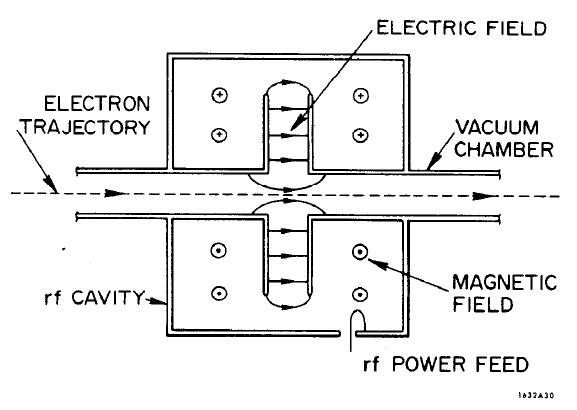
\includegraphics[width=0.7\linewidth]{./Figuras/fig30.jpeg}
	\caption{Diagrama esquemático de uma cavidade de RF. Retirado de \cite{sands1970physics}.}
	\label{fig:fig30}
\end{figure}

Como os campos de RF variam com o tempo, a energia recebida por um elétron em uma revolução depende do tempo em que este elétron passou pela cavidade de RF. Suponha que a dependência temporal do campo elétrico é dada. Então a energia $U_{RF}$ recebida por um elétron em uma revolução irá depender do tempo $\bar{t}$ em que ele começou sua revolução (considerando uma coordenada $s$ de referência, suponha $s=0$).

Se os elétrons devem ser armazenados próximos à órbita ideal, a variação de $U_{RF}(\bar{t})$ deve possuir algumas características. Primeiramente, assume-se que $U_{RF}(\bar{t})$ é uma função periódica com um período submúltiplo de $T_0$, o período de uma revolução de um elétron circulando na órbita ideal. Ou seja,
\begin{align}
	U_{RF}(\bar{t}+T_0/k) = U_{RF}(\bar{t})\label{eq:3.25}
\end{align}
onde $k$ é um inteiro chamado de número harmônico do sistema de RF. A variação de $U_{RF}(\bar{t})$ pode ser, por exemplo, como a curva representada na \autoref{fig:fig31} (apesar da suposição sobre a variação temporal de $U_{RF}$ ser mais restritiva que o necessário, os campos de RF devem ter pelo menos características similares para que o anel de armazenamento funcione).

\begin{figure}[!htb]
	\centering
	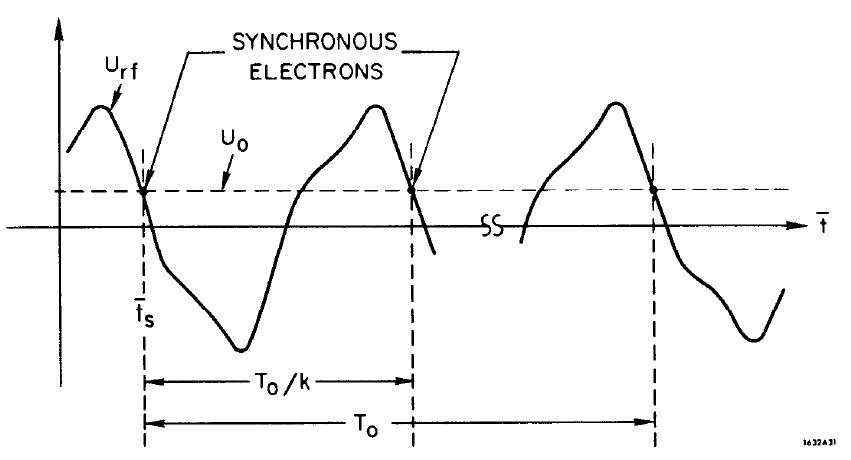
\includegraphics[width=0.85\linewidth]{./Figuras/fig31.jpeg}
	\caption{Ganho de energia do sistema de RF como uma função do tempo inicial $t$ de uma revolução. Retirado de \cite{sands1970physics}.}
	\label{fig:fig31}
\end{figure}

Agora, considere o que pode acontecer com um elétron com energia nominal $E_0$ circulando pela órbita ideal. Suponha que sua trajetória iniciou em $\bar{t}_s$, exatamente o tempo em que $U_{RF}(\bar{t}_s) = U_0$. Veja a \autoref{fig:fig31}. Na próxima revolução, perda e ganho de energia irão se compensar e o elétron irá retornar para seu ponto inicial novamente com energia $E_0$. O tempo necessário para uma revolução é $T_0$: então o elétron irá começar a próxima revolução no tempo $\bar{t}_s + T_0$ e, pela equação \eqref{eq:3.25}, o ganho de RF será novamente igual a $U_0$. O elétron irá continuar circulando pela órbita ideal indefinidamente. Este elétron o qual passa a coordenada de referência em $\bar{t}_s+jT_0$ (onde $j=1,2,3,...$) é chamado de elétron síncrono -- porque sua rotação está sincronizada com os campos de RF oscilantes. E $\bar{t}_s$ é chamada de fase síncrona do sistema de RF (é claro que com um sistema de Rf periódico existem tempos de início síncronos equivalentes para cada período de RF).

Foi assumido que o valor de pico de $U_{RF}$ é maior que a perda por radiação $U_0$ de um elétron síncrono. Disso, segue que existem ao menos duas escolhas possíveis de $\bar{t}_s$ em cada ciclo de $U_{RF}$ -- um onde $U_{RF}$ é crescente e outro onde ela é decrescente. Apenas um dos dois -- aquele onde $U_{RF}$ decresce -- corresponde a um movimento estável, como será mostrado. Então apenas este será designado como a fase síncrona $\bar{t}_s$. Pela \autoref{fig:fig31} também pode-se observar que com um número harmônico $k$ existem $k$ tempos síncronos de início diferentes -- e, desta forma, $k$ elétrons síncronos. Estas $k$ fases síncronas correspondem aos $k$ possíveis \textit{bunches}de elétrons armazenados no anel.

Um elétron movendo-se com um deslocamento lateral com relação á órbita ideal irá ver um campo elétrico diferente do campo visto por um elétron na órbita ideal. Porém, geralmente o ganho de energia em uma revolução depende muito pouco do deslocamento lateral. Sendo assim, é razoável ignorar qualquer dependência do ganho de energia com o deslocamento lateral -- independente se este for causado por oscilações betatron ou de energia -- e considerar apenas a variação do ganho de energia com o tempo de início $\bar{t}$.

A posição circular do elétron síncrono prevê um ponto de referência conveniente para o estudos das oscilações longitudinais de um elétron em um \textit{bunch}. De fato, esta posição  do elétron síncrono é referenciada como sendo o "centro"  do \textit{bunch} e descreve a posição azimutal instantânea de qualquer outro elétron do \textit{bunch} em função do seu deslocamento longitudinal $y$ a partir do centro do \textit{bunch}. Isto é, define-se
\begin{align}
	y(t) = s(t) - s_c(t)
\end{align}
onde $s$ é a posição azimutal de qual elétron em particular e $s_c$ refere-se a posição do centro do \textit{bunch}. Veja a \autoref{fig:fig32}.

\begin{figure}[!htb]
	\centering
	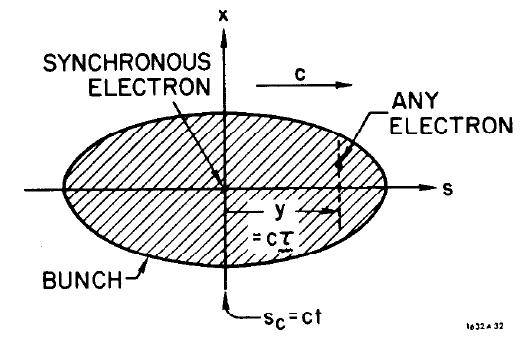
\includegraphics[width=0.6\linewidth]{./Figuras/fig32.jpeg}
	\caption{Coordenadas longitudinais $y$ e $\tau$ de um elétron em um \textit{bunch}. Retirado de \cite{sands1970physics}.}
	\label{fig:fig32}
\end{figure}

Para a presente discussão, é conveniente descrever o movimento longitudinal por uma variável equivalente $\tau$ definida simplesmente como
\begin{align}
	\tau(t) = y(t)/c
\end{align}
e chamada de deslocamento temporal do centro do \textit{bunch}. O deslocamento temporal é muito próximo do intervalo de tempo $\Delta t$ entre a chegada de um elétron em qualquer coordenada $s$ em particular e a chegada do elétron síncrono nesta mesma coordenada. A diferença é igual a mudança em $\tau$ no tempo $\Delta t = \tau$, a qual pode ser ignorada devido a lenta variação de $\tau$. note que o deslocamento temporal $\tau$ é positivo quando um elétron chega em cada coordenada $s$ antes do elétron síncrono.

Devido às variações temporais dos campos elétricos do sistema de RF, apenas um elétron síncrono irá receber a energia $U_0$ em uma revolução. Qualquer outro elétron irá ganhar uma energia $U_{RF}$ que depende do deslocamento temporal $\tau$. Utilizando a notação convencional, escreve-se
\begin{align}
	U_{RF} = eV(\tau)
\end{align}
onde $e$ é a carga do elétron e $V(\tau)$ é chamada de "tensão de RF" -- em analogia a um sistema de aceleração DC. A forma de $V(\tau)$ é, claro, relacionada a $U_{RF}$; especificamente,
\begin{align}
	eV(\tau) = U_{RF}(\bar{t}_s - \tau)
\end{align}
A variação com relação a $\tau$ é contrário à variação com $\bar{t}$, então a função de ganho de energia dada pela \autoref{fig:fig31} corresponde à função $V(\tau)$ dada pela \autoref{fig:fig33} -- onde, agora, $\tau=0$ corresponde ao deslocamento temporal de um elétron síncrono. Note que a inclinação de $V(\tau)$ é positiva em $\tau=0$.

\begin{figure}[!htb]
	\centering
	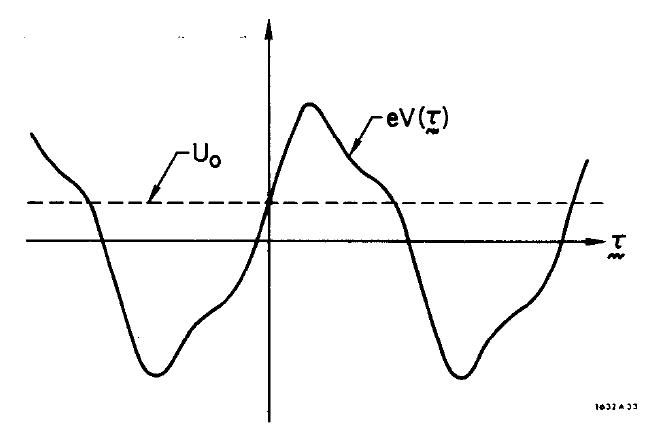
\includegraphics[width=0.6\linewidth]{./Figuras/fig33.jpeg}
	\caption{Função da tensão de RF $V(\tau)$. Retirado de \cite{sands1970physics}.}
	\label{fig:fig33}
\end{figure}

É pertinente enfatizar o fato de que a "tensão" efetiva de múltiplas cavidades de RF de anéis de armazenamento de alta energia não é simplesmente relacionada com alguma "tensão" elétrica observável, mas esta sim depende das posições relativas e fases de oscilação das várias cavidades de Rf do sistema. A tensão $V(\tau)$ depende, na verdade, do sentido de circulação da partícula ao redor do anel e, sendo assim, pode ser diferente para elétrons circulando em um sentido ao redor do anel e positróns circulando no sentido contrário.

Agora, as oscilações de energia de um elétron em um \textit{bunch} circulando no anel de armazenamento estão prontas para serem consideradas. Primeiramente, pode-se fazer uma análise qualitativa do que irá acontecer. Suponha que o elétron comece com energia nominal $E_0$, mas com um deslocamento temporal positivo $\tau$ -- desta forma, o elétron está à frente da posição síncrona. A perda por radiação depende apenas da energia, então ela será $U_0$ a cada revolução. Mas o ganho de energia será maior que $U_0$, uma vez que o elétron está adiantado com relação ao elétron síncrono. Este elétron ganhará um pouco mais de energia a cada revolução. Mas um aumento na sua energia irá, pela equação \eqref{eq:3.15}, causar um aumento no seu período de revolução; e seu avanço de tempo com relação ao centro do \textit{bunch} irá, portanto, começar a diminuir. Após algumas revoluções, o deslocamento temporal chegará a zero. Mas, quando isto acontecer, a energia do elétron será maior que a energia nominal $E_0$ -- já que ele esteve ganhando energia continuamente -- então seu deslocamento temporal continuará diminuindo, agora assumindo valores negativos de $\tau$. No entanto, em valores negativos de $\tau$, o ganho de energia será muito pequeno para compensar a perda de energia por radiação e a energia do elétron irá começar a diminuir em direção à energia nominal $E_0$. Quando a energia nominal for atingida, o deslocamento temporal irá parar de diminuir mas, como $\tau$ é negativo, o ganho de energia por revolução é menor que $U_0$ e a energia irá começar a decrescer, ficando menor que $E_0$. Agora o deslocamento temporal irá começar a aumentar, voltando para zero. O processo irá continuar até que $\tau$ retorne ao seu valor inicial, onde a energia será novamente $E_0$.

Analisando agora de forma quantitativa. Primeiramente, analise a variação do deslocamento temporal $\tau$. É conveniente analisar o que está acontecendo observando um \textit{bunch} a cada revolução quando o centro do \textit{bunch} está em alguma coordenada de referência. A discussão é facilitada tomando esta coordenada de referência em um ponto sem nenhum campo (longe de ímãs ou cavidades de RF). Na \autoref{fig:fig34} estão contidas duas "fotos" do mesmo \textit{bunch} em duas passagens consecutivas pela coordenada de referência. Em cada foto o centro do \textit{bunch} está na coordenada de referência, então o tempo entre as imagens é apenas $T_0$ --  o tempo de uma revolução pela órbita ideal.

\begin{figure}[!htb]
	\centering
	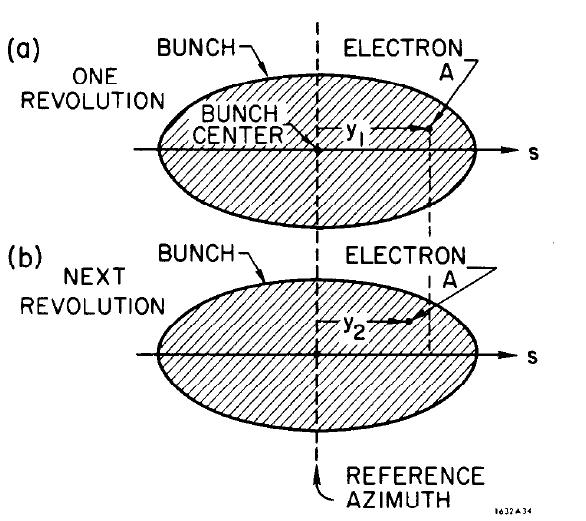
\includegraphics[width=0.6\linewidth]{./Figuras/fig34.jpeg}
	\caption{Movimento longitudinal de um elétron em um \textit{bunch}. Retirado de \cite{sands1970physics}.}
	\label{fig:fig34}
\end{figure}

As imagens também mostram a posição de um elétron em particular: "Elétron A". Na primeira imagem, o Elétron A está à frente do centro do \textit{bunch} de uma distância $y_1$. Na segunda imagem, o deslocamento longitudinal decaiu para $y_2$. Entre as duas "fotos", o centro do \textit{bunch} percorreu uma volta ao longo da órbita ideal, ou seja, uma distância $L=cT_0$. E, como o Elétron A também viaja na velocidade da luz $c$, este também percorreu uma distância $L$. Mas, se este elétron possui um desvio de energia $\epsilon$, foi mostrado na \autoref{sec:3.2} que o comprimento de uma revolução completa será maior que $L$ por uma quantidade $\delta \ell$ dada por
\begin{align}
	\frac{\delta \ell}{L} = \alpha\frac{\epsilon}{E_0}
\end{align}
Note que para $\epsilon$ positivo -- ou seja, $E>E_0$ -- $\delta \ell$ também é positivo, o que implica que o caminho a ser percorrido pelo elétron fica maior. Pois bem, desta forma o Elétron A não consegue alcançar sua coordenada anterior $y_1$ por uma pequena distância $\delta y = -\delta \ell$, ou seja,
\begin{align}
	y_2 - y_1 = \delta y = -\alpha \frac{\epsilon}{E_0}L
\end{align}
A variação de $\tau$ em uma revolução é
\begin{align}
	\delta \tau = \frac{\delta y}{c} = -\alpha \frac{\epsilon}{E_0}\frac{L}{c} = -\alpha\frac{\epsilon}{E_0}T_0
\end{align}
Como o tempo entre cada imagem é $T_0$, a taxa de variação temporal de $\tau$ é apenas $\delta \tau/T_0$, ou ainda
\begin{align}
	\frac{d \tau}{dt} = -\alpha \frac{\epsilon}{E_0}\label{eq:3.32}
\end{align}

Agora, a variação da energia. Durante sua revolução, o Elétron A perdeu uma parte $U_{rad}(\epsilon)$ da sua energia, e ganhou da cavidade de RF $eV(\tau_1)$. A variação da energia nesta revolução é, portanto,
\begin{align}
	\delta U = eV(\tau)-U_{rad}(\epsilon)
\end{align}
A taxa de variação do desvio de energia $\epsilon$ -- avaliada em uma revolução completa -- é $\delta U/T_0$, então tem-se que
\begin{align}
	\frac{d\epsilon}{dt} = \frac{eV(\tau)-U_{rad}(\epsilon)}{T_0}\label{eq:3.34}
\end{align}

Combinando as equações \eqref{eq:3.32} e \eqref{eq:3.34}, pode-se descrever as oscilações de energia -- e as oscilações temporais associadas --  de um elétron armazenado. É preciso resolver as duas equações juntas para obter a variação de $\epsilon$ e $\tau$ com relação ao tempo.

Infelizmente, os deslocamentos temporais associados a pequenas variações de energia não são necessariamente pequenos no sentido de eles podem abranger uma fração significante de um ciclo completo de variação de $V(\tau)$. Apenas neste caso não é possível considerar apenas os termos lineares durante a análise. Talvez seja necessário computar as variações não-lineares de $V(\tau)$. Nos casos em que uma pequena variação da energia causa um deslocamento temporal é pequeno, entretanto, pode-se considerar apenas os termos lineares da variação de $V(\tau)$. Já que o ganho de energia para $\tau=0$ é, por definição, $U_0$, ao expandir a função em série de Taylor tem-se que
\begin{align}
	U_{RF} = eV(\tau) = U_0 + e\dot{V}_0\tau\label{eq:3.35}
\end{align}
onde $\dot{V}_0$ é $dV/d\tau$ avaliada em $\tau=0$.

É comum que a tensão de Rf em um anel de armazenamento tenha uma variação senoidal com relação ao tempo. Nestes casos, tem-se que a tensão é descrita por
\begin{align}
	V(\tau) = \widehat{V}\ sen(\omega_{RF}(\tau+\tau_0))
\end{align}
onde $\widehat{V}$ é chamado de valor de pico da tensão de RF e $\omega_{RF}\tau_0$ é chamada de fase síncrona de RF. De acordo com as suposições feitas,
\begin{align}
	\omega_{RF} = 2\pi \frac{k}{T_0} = k\omega_r
\end{align}
onde $\omega_r$ é a frequência angular de uma revolução. Também segue que
\begin{align}
	\omega_{RF}\tau_0 = sen^{-1}(U_0/e\widehat{V})
\end{align}
e
\begin{align}
	\dot{V}_0 = \omega_{RF}\widehat{V}cos(\omega_{RF}\tau_0) = \omega_{RF}\widehat{V}\left[1-\left(\frac{U_0}{e\widehat{V}}\right)^2\right]^{1/2}
\end{align}

\begin{proof}
	Pela equação \eqref{eq:3.25}, o período da função $U_{RF}$ é $T_0/k$. Logo, sua frequência é $k/T_0$. Logo, sua frequência angular é
	\begin{align*}
		\omega_{RF} = 2\pi f_{RF} = 2\pi \frac{k}{T_0}
	\end{align*}
	Mas $2\pi \frac{1}{T_0}$ é a frequência angular de uma revolução completa. Logo, $\omega_{RF} = k\omega_r$.
	
	Agora, seja a tensão de RF dada por $V(\tau) = \widehat{V}\ sen(\omega_{RF}(\tau+\tau_0))$. Logo, $V(0) = \widehat{V}\ sen(\omega_{RF}\tau_0)$. Sendo assim, avaliando a equação \eqref{eq:3.35} em $\tau=0$, tem-se que
	\begin{align*}
		e\widehat{V}\ sen(\omega_{RF}\tau_0) &= U_0\\
		\therefore \omega_{RF}\tau_0 &= sen^{-1}(U_0/e\widehat{V})
	\end{align*}
	Por fim, derivando a expressão de $V(\tau)$, tem-se
	\begin{align*}
		\frac{dV}{d\tau} &= \omega_{RF}\widehat{V}\ cos(\omega_{RF}(\tau+\tau_0))\\
		\therefore \widehat{V}_0 = \left(\frac{dV}{d\tau}\right)_0 &= \omega_{RF}\widehat{V}\ cos(\omega_{RF}(\tau_0))
	\end{align*}
	Mas, pela relação trigonométrica $sen^2(x) + cos^2(x) = 0$, tem-se que
	\begin{align*}
		cos(\omega_{RF}\tau_0) = [1-sen^2(\omega_{RF}\tau_0)]^{1/2}\\
		\therefore \widehat{V}_0 = \omega_{RF}\widehat{V}[1-sen^2(\omega_{RF}\tau_0)]^{1/2}
	\end{align*}
	Porém, já foi demonstrado aqui que $\omega_{RF}\tau_0 = sen^{-1}(U_0/e\widehat{V})$. Substituindo esta relação, tem-se que
	\begin{align*}
		\therefore \widehat{V}_0 = \omega_{RF}\widehat{V}\left[1-\left(\frac{U_0}{e\widehat{V}}\right)\right]^{1/2}
	\end{align*}
	c.q.d.
\end{proof}